\section{Introductie}

% \subsection[Introduction]{Introduction Masterclass GR-Advanced}

\begin{frame} %TODO: Variable over time
\frametitle{Let me introduce myself\ldots}

\begin{itemize}
  \item Kevin van As (23yr)
  \pause
  \item PhD aan de TUDelft in de Natuurkunde
  \pause
  \item Hobbies:
  \begin{itemize}
  	\item Les geven
  	\item Masterclasses organiseren
  	\pause
  	\item Computer programmeren
  	\pause
  	\item Computer games
  \end{itemize}
\end{itemize}
\end{frame}

\begin{frame}
\frametitle{Wat is de cursus?}
\framesubtitle{Leerdoelen}

Je zult leren:
\begin{itemize}
  \item Je Grafische Rekenmachine (GR) TI-84 beter leren kennen.
  \pause
  \item Leren om programma's (\tiPRGM) voor de GR te schrijven:
  \pause
  \begin{itemize}
    \item ABC-formule
    \pause
    \item Priemgetallen
    \pause
    \item Oplossen van (willekeurige) functies
    \pause
    \item Grafisch bewerken van functies
    \pause
    \item Eenheidscirkel
    \pause
    \item Exactor
  \end{itemize}
  \pause
  \item En dit leert je ook inzichten om op de computer te leren programmeren!
\end{itemize}
	
\begin{picture}(1,1)
  	\put(240,43){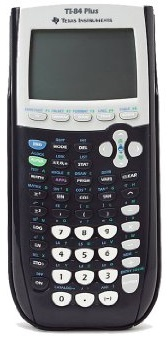
\includegraphics[height=0.3\textheight]{TI84.jpg}}
\end{picture}
\end{frame}

\begin{frame}
\frametitle{Opzet cursus}

\begin{itemize} %TODO: Variable over time
  \item Wekelijks op Maandagavond 19:00-21:00.
  \pause
  \item Van DD/MM/YY tot DD/MM/YY, in totaal 6 keer.
  \pause
  \item Les bestaat uit beetje uitleg, en veel zelf proberen.
  \pause
  \item Je krijgt opdrachten mee naar huis om zelf te oefenen.
\end{itemize}

\end{frame}

\begin{frame}
\frametitle{Notatie op deze slides}

Op deze slides zullen we drie verschillende lettertypen vinden.
Het huidige lettertype is normale tekst.

\pause
\tifonttxt{Dit lettertype wordt gebruikt om tekst van je rekenmachine te laten zien.} \inlineticalc{7 \> A: A \! 6}

\pause
Tekens als \tiPRGM, \tiGRAPH, \tiCOS,  \tiXTn\, en \tiENTER\, zijn fysieke knoppen van je rekenmachine.

\pause
En tekens als \tiLOne, \tiACOS, en \tiMATRIX\, zijn knoppen die je met \tiSecond\, kunt bereiken.
Deze knoppen staan boven andere knoppen. Bijvoorbeeld \tiTEST\, is gelijk aan \tiSecond\tiMATH.

\vspace{10 mm}
\visible<5->{
Nu\ldots Laten we beginnen! Rekenmachines bij de hand\ldots
}
\end{frame}


%% END %%